

\section{Project organization}

\subsection{Project organization}
We have decided to use the Scrum model for organizing our group. This means that we have a flat organizational structure where everyone contributes with what they can. Even in a flat structure, it is important to share responsibilities, so each person of the group has a main focus area. If it is too much work for a person, it is important that the work is delegated to the others.

\subsection{Organizational diagram}
See figurel \ref{fig:organizationalchart} at page \pageref{fig:organizationalchart}
\begin{figure}
\begin{center}
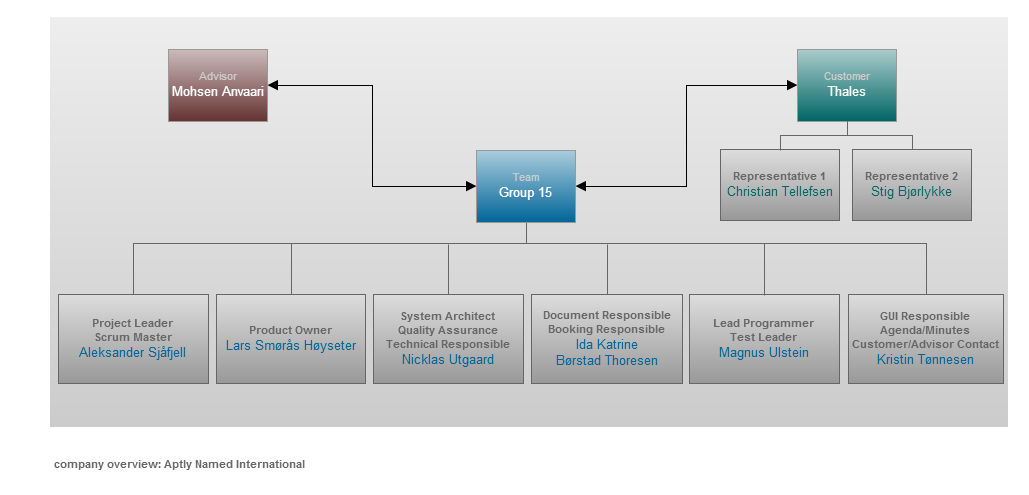
\includegraphics[width=\textwidth]{Organizational_Chart_v2}
\caption{Organizational chart} \label{fig:organizationalchart}
\end{center}
\end{figure}

\subsection{Role allocation}
See tabel \ref{tab:roleallocation} at page \pageref{tab:roleallocation}
\begin{table}
\begin{tabularx}{\linewidth}{>{\setlength\hsize{.5\hsize}}X|>{\setlength\hsize{0.3\hsize}}X|>{\setlength\hsize{1\hsize}}X}
\textbf{Role} & \textbf{Person} & \textbf{Responsibilities} \\ \hline \hline
Project leader & Aleksander & Make sure everybody does what they are supposed to and peacefully resolve disputes between participants. \\ \hline
Scrum master & Aleksander & Make sure the team’s work conform to Scum standards and help the team do the best work possible. \\ \hline
Booking of rooms & Ida & Booking rooms for the meetings and other activities. \\ \hline
Agendas, minutes of meetings & Kristin \& Lars &Write agendas and minutes of meeting and send these out within the specified time limits. \\ \hline
Customer/advisor contact & Kristin & Main contact person for customer and advisor. \\ \hline
Document responsible & Ida &Keep track of what is to be contained in the project report, what has been written and what remains. \\ \hline
Project report layout responsible & Ida &Find programs to make tables and graphs, and check that all diagrams are similar ib style. \\ \hline
System architect & Nicklas & Defining the system architecture. \\ \hline
Test leader & Magnus & Lead the testing team. \\ \hline
Technical responsible & Nicklas & Setup of Netbeans, Git and other tools that the team uses in the development. \\ \hline
Quality assurance responsible & Nicklas & Make sure that all routines, templates and standards are followed. \\ \hline
Responsible for graphical user interface & Kristin & Design the views and the interactions and setting up the MVC structure. \\ \hline
Lead programmer & Magnus & Responsible for having a general overview of the code. This means knowing what is to be implemented next, and seeing that this is done at the right time. \\ \hline
Product owner & Lars & Represent the stakeholder and ensure that the team delivers value to businesses.
\end{tabularx}
\caption {Role allocation} \label{tab:roleallocation}
\end{table}

\subsection{Weekly schedule}
See tabel \ref{tab:weeklyschedule} at page \pageref{tab:weeklyschedule}
\begin{table}
\begin{tabular}{l|l|l|l|l|l}
 & \textbf{Monday} & \textbf{Tuesday} & \textbf{Wednesday} & \textbf{Thursday} & \textbf{Friday} \\ \hline \hline
\textbf{08-09} &  & Group work &  &  &  \\ \hline
\textbf{09-10} &  & Group work &  &  &  \\ \hline
\textbf{10-11} &  & Group work &  &  &  \\ \hline
\textbf{11-12} &  & Advisor meeting & &  &  \\ \hline
\textbf{12-13} & Group work & Group work & Customer meeting &  &  \\ \hline
\textbf{13-14} & Group work & Group work & Group work &  &  \\ \hline
\textbf{14-15} & Group work & Group work & Group work &  &  \\ \hline
\textbf{15-16} & Group work &  & Group work &  &  \\ \hline
\textbf{16-17} & Group work &  & Group work &  &  \\ \hline
\textbf{17-18} & Group work &  & Group work &  & 
\end{tabular}
\caption {Weekly schedule} \label{tab:weeklyschedule}
\end{table}

